\documentclass[
10pt, % Main document font size
a4paper, % Paper type, use 'letterpaper' for US Letter paper
oneside, % One page layout (no page indentation)
%twoside, % Two page layout (page indentation for binding and different headers)
headinclude,footinclude, % Extra spacing for the header and footer
BCOR5mm, % Binding correction
]{scrartcl}

\usepackage{listings}
\usepackage{color}
%\usepackage{biblatex}

\definecolor{dkgreen}{rgb}{0,0.6,0}
\definecolor{gray}{rgb}{0.5,0.5,0.5}
\definecolor{mauve}{rgb}{0.58,0,0.82}

\lstset{frame=tb,
	language={},
	aboveskip=3mm,
	belowskip=3mm,
	showstringspaces=false,
	columns=flexible,
	basicstyle={\small\ttfamily},
	numbers=none,
	numberstyle=\tiny\color{gray},
	keywordstyle=\color{blue},
	commentstyle=\color{dkgreen},
	stringstyle=\color{mauve},
	breaklines=true,
	breakatwhitespace=true,
	tabsize=3
}

\usepackage{german}


%usepackage[utf8]{inputenc}
%\usepackage{geometry}
\usepackage[german,onelanguage,linesnumbered, ruled]{algorithm2e}
\SetAlFnt{\small}
\SetAlCapFnt{\large}
\SetAlCapNameFnt{\large}
%\usepackage{algpseudocode}


%%%%%%%%%%%%%%%%%%%%%%%%%%%%%%%%%%%%%%%%%
% Arsclassica Article
% Structure Specification File
%
% This file has been downloaded from:
% http://www.LaTeXTemplates.com
%
% Original author:
% Lorenzo Pantieri (http://www.lorenzopantieri.net) with extensive modifications by:
% Vel (vel@latextemplates.com)
%
% License:
% CC BY-NC-SA 3.0 (http://creativecommons.org/licenses/by-nc-sa/3.0/)
%
%%%%%%%%%%%%%%%%%%%%%%%%%%%%%%%%%%%%%%%%%

%----------------------------------------------------------------------------------------
%	REQUIRED PACKAGES
%----------------------------------------------------------------------------------------

\usepackage[
nochapters, % Turn off chapters since this is an article        
beramono, % Use the Bera Mono font for monospaced text (\texttt)
eulermath,% Use the Euler font for mathematics
pdfspacing, % Makes use of pdftex’ letter spacing capabilities via the microtype package
dottedtoc % Dotted lines leading to the page numbers in the table of contents
]{classicthesis} % The layout is based on the Classic Thesis style

\usepackage{arsclassica} % Modifies the Classic Thesis package

\usepackage[T1]{fontenc} % Use 8-bit encoding that has 256 glyphs

\usepackage[utf8]{inputenc} % Required for including letters with accents

\usepackage{graphicx} % Required for including images
\graphicspath{{Figures/}} % Set the default folder for images

\usepackage{enumitem} % Required for manipulating the whitespace between and within lists

\usepackage{lipsum} % Used for inserting dummy 'Lorem ipsum' text into the template

\usepackage{subfig} % Required for creating figures with multiple parts (subfigures)

\usepackage{amsmath,amssymb,amsthm} % For including math equations, theorems, symbols, etc

\usepackage{varioref} % More descriptive referencing

%----------------------------------------------------------------------------------------
%	THEOREM STYLES
%---------------------------------------------------------------------------------------

\theoremstyle{definition} % Define theorem styles here based on the definition style (used for definitions and examples)
\newtheorem{definition}{Definition}

\theoremstyle{plain} % Define theorem styles here based on the plain style (used for theorems, lemmas, propositions)
\newtheorem{theorem}{Theorem}

\theoremstyle{remark} % Define theorem styles here based on the remark style (used for remarks and notes)

%----------------------------------------------------------------------------------------
%	HYPERLINKS
%---------------------------------------------------------------------------------------

\hypersetup{
%draft, % Uncomment to remove all links (useful for printing in black and white)
colorlinks=true, breaklinks=true, bookmarks=true,bookmarksnumbered,
urlcolor=webbrown, linkcolor=RoyalBlue, citecolor=webgreen, % Link colors
pdftitle={}, % PDF title
pdfauthor={\textcopyright}, % PDF Author
pdfsubject={}, % PDF Subject
pdfkeywords={}, % PDF Keywords
pdfcreator={pdfLaTeX}, % PDF Creator
pdfproducer={LaTeX with hyperref and ClassicThesis} % PDF producer
} % Include the structure.tex file which specified the document structure and layout

\hyphenation{Fortran hy-phen-ation} % Specify custom hyphenation points in words with dashes where you would like hyphenation to occur, or alternatively, don't put any dashes in a word to stop hyphenation altogether

%----------------------------------------------------------------------------------------
%	TITLE AND AUTHOR(S)
%----------------------------------------------------------------------------------------

\title{\normalfont\spacedallcaps{Projektaufgabe AE}} % The article title

\subtitle{Remove Duplicates - Spotify playlist cleaner} % Uncomment to display a subtitle

\author{\spacedlowsmallcaps{Raphael Drechsler}} % The article author(s) - author affiliations need to be specified in the AUTHOR AFFILIATIONS block

\date{} % An optional date to appear under the author(s)

%----------------------------------------------------------------------------------------

\begin{document}

%----------------------------------------------------------------------------------------
%	HEADERS
%----------------------------------------------------------------------------------------

\renewcommand{\sectionmark}[1]{\markright{\spacedlowsmallcaps{#1}}} % The header for all pages (oneside) or for even pages (twoside)
%\renewcommand{\subsectionmark}[1]{\markright{\thesubsection~#1}} % Uncomment when using the twoside option - this modifies the header on odd pages
\lehead{\mbox{\llap{\small\thepage\kern1em\color{halfgray} \vline}\color{halfgray}\hspace{0.5em}\rightmark\hfil}} % The header style

\pagestyle{scrheadings} % Enable the headers specified in this block

%----------------------------------------------------------------------------------------
%	TABLE OF CONTENTS & LISTS OF FIGURES AND TABLES
%----------------------------------------------------------------------------------------

\maketitle % Print the title/author/date block

\setcounter{tocdepth}{2} % Set the depth of the table of contents to show sections and subsections only

\tableofcontents % Print the table of contents

%\listoffigures % Print the list of figures

%\listoftables % Print the list of tables




%----------------------------------------------------------------------------------------

\newpage % Start the article content on the second page, remove this if you have a longer abstract that goes onto the second page

%----------------------------------------------------------------------------------------
%	INTRODUCTION
%----------------------------------------------------------------------------------------
\section{Problemstellung ''Remove Duplicates''}

\textbf{Problem}\\
Gegeben ist eine Sequenz. Diese Sequenz enthält ggf. Duplikate. \\
Ziel des umzusetzenden Algorithmus ist das Entfernen der Duplikate aus dieser Sequenz.\\

Für die Umsetzung eines entsprechenden Algorithmus sollen die zwei folgenden Ansätze betrachtet werden:
\begin{itemize}[noitemsep]
	\item Naiver Ansatz: Nutzung eines einfachen Arrays
	\item Ansatz im Fokus: Nutzung einer Hash-Table
\end{itemize}\

\textbf{Naiver Ansatz}\\
In der Implementierung nach dem naiven Ansatz würden alle Daten einer Sequenz in einem Array gespeichert werden, insofern sie nicht bereits im Array enthalten sind. Beim betrachten eines Elementes aus der Sequenz muss also in der naiven Umsetzung das komplette Array nach einem identischen Element durchsucht werden. Im in Hinblick auf die Laufzeit schlimmsten Fall, muss daher jedes Element im Array mit dem aktuell untersuchten Element des Sequenz verglichen werden. Bei einer Sequenz-Liste der Größe \(n\) müssen also im wors-case 
\begin{equation}
	\sum_{k=1}^{n-1} k
\end{equation}
Vergleichsoperationen durchgeführt werden. Betrachtet man die folgende Umformung entsprechend der Gaußschen Summenformel
\begin{equation}
	\sum_{k=1}^{n-1} k = \frac{(n-1)^2 + (n-1)}{2} = \frac{1}{2} (n-1)^2
\end{equation}


ergibt sich für eine Umsetzung dieses Ansatzes eine theoretische obere Komplexitätsgrenze von 

\begin{equation}
O(n^2)
\end{equation}


\textbf{Ansatz Hash-Table}\\
Der Ansatz ''Hash-Table'' setzt an dem Punkt der Komplexitätsbetrachtung an\\
Würde man für die Einordnung der Elemente in das Array eine Direktadressierung verwenden, so würde man ein Element selbst als Schlüssel interpretieren, mit dem ein Feld im Array adressiert wird.

\begin{figure}[h]
	\centering 
	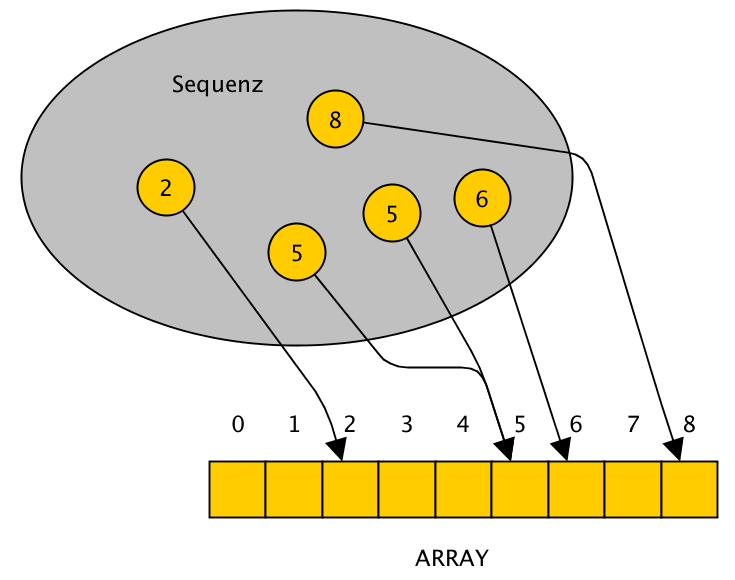
\includegraphics[width=0.5\columnwidth]{Diag1} 
	\caption[Skizze Direkte Adressierung]{Skizze: Prinzip der direkten Adressierung \textit{nach} \cite{Cormen:2009:IAT:1614191}}
	
\end{figure}

Der Zeitaufwand für die Prüfung, ob ein Element bereits im Array gespeichert ist, wäre dabei \(O(1)\).\\
Ist das Universum \(U={0,1,...,m}\), in denen sich die Schlüssel der Elemente befinden klein, lässt sich somit schnell auf ein Array der Größe \(A[0..m-1]\) zugreifen. Ab einer bestimmten Größe des Universums kann eine Umsetzung der Direkt-Adressierung Aufgrund der erforderlichen Größe des Ziel-Arrays nicht mehr sinnvoll bzw. möglich sein.\\
Die Hash-Table löst dieses Problem, indem sie das große Universum \(U\) einem kleineren Array \(A[0..m-1]\) gegenüberstellt. Die Adressierung der Array-Felder pro Element erfolgt weiterhin auf Grundlage des Element-Wertes. Um nur existierende Schlüssel zu erhalten wird zur Ermittlung des Schlüssels eine Funktion \(h\) (sogenannte Hash-Funktion) eingesetzt, welche die Werte der Elemente im Universum \(U\) auf existierende Schlüssel abbildet. \textit{vgl.}\cite{Cormen:2009:IAT:1614191}
\begin{equation}
h: U-> {0,...,m-1}
\end{equation}\
Die Skizze gestaltet sich wie folgt:\\
\begin{figure}[h!]
	\centering 
	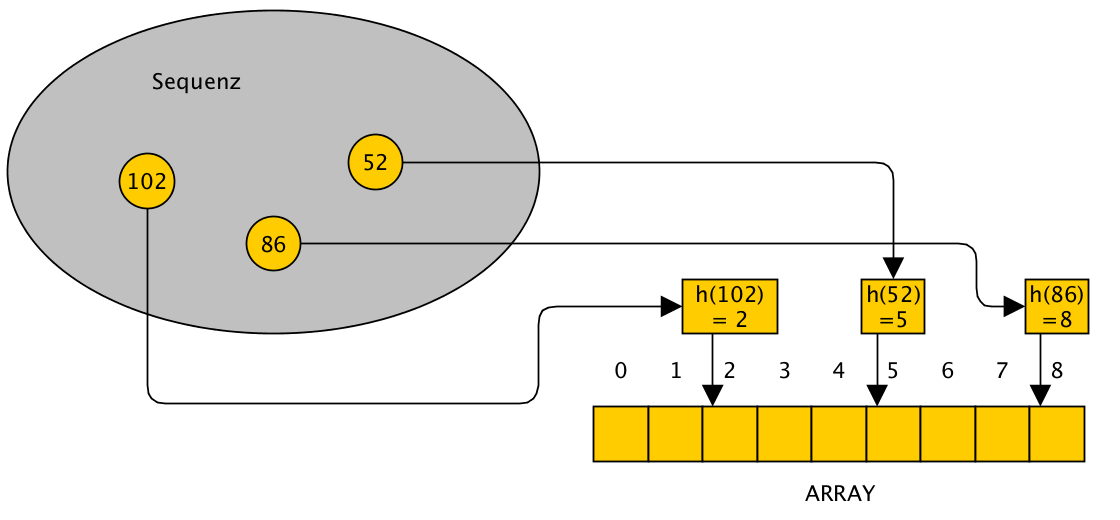
\includegraphics[width=0.75\columnwidth]{Diag2} 
	\caption[Skizze Adressierung in Hash-Table]{Skizze: Prinzip der Adressierung in einer Hash-Table\textit{nach} \cite{Cormen:2009:IAT:1614191}}
	
\end{figure}\

Dadurch, dass gilt \(|U|>m\) wird über Anwendung des Schubfachprinzips ersichtlich, dass die Hash-Funktion \(h\) nicht injektiv ist. \\
Fälle in denen gilt
\begin{equation}
h(a)=h(b)|a,b\in U, a\neq b
\end{equation}
werden als Kollision bezeichnet. \textit{vgl.}\cite{Cormen:2009:IAT:1614191}\\
Bei der Umsetzung des Algorithmus muss also eine entsprechende Strategie zur Auflösung solcher Kollisionen mit betrachtet werden.\\

\textbf{Kollisions-Auflösung im python dict-Objekt}\\
Als Kollisions-Auflösungs-Strategie soll im Rahmen der Umsetzung das Verfahren implementiert werden, welches im python-Standard beim Zugreifen auf \textit{dict}-Objekte genutzt wird. Durch die ggf. notwendige Behandlung von Kollisionen ergibt sich für einen Zugriff auf ein Feld des Arrays bei einer entsprechenden Implementierung der folgende Zeitbedarf.

\begin{table}[h!]
	\centering 
	\begin{tabular}{l|c|c|c|c|c|}
		\hline 
		Operation & average-case & worst-case \\ 
		\hline 
		Element einfügen & \(O(1)\) & \(O(n)\)\\
		\hline 
		Auf Element zugreifen & \(O(1)\) & \(O(n)\)\\
	\end{tabular}\\
	\caption[Zugriffs-Komplexität im python dict]{Zugriffs-Komplexität im python dict \cite{TimeComplexityPy}}
\end{table}\

\section{Anwendungsszenario Spotify Playlists}
Als Anwendungsfall soll das disjunkte Vereinigen von Titeln mehrerer Spotify-Playlists betrachtet werden.\\
In Spotify lassen sich für eine geöffnete Playlist per Tastatur-Kurzbefehl ''Strg + A'' und ''Strg + C'' alle Titel der Playlist in die Zwischenablage kopieren. Die Titel werden dabei als URI repräsentiert.

\begin{figure}[h!]
	\centering 
	\begin{lstlisting}
	https://open.spotify.com/track/757530vPBymdi31CtXstxP
	https://open.spotify.com/track/1Qi256uJuMihknGuuFcQoC
	https://open.spotify.com/track/0JFBf2PloRfMkPg5DjXhDx
	https://open.spotify.com/track/7iXF2W9vKmDoGAhlHdpyIa
	\end{lstlisting}
	\caption[Beispiel Spotify-Titel URIs]{Beispiel: Spotify-Titel URIs}
\end{figure}\

Die URIs werden durch den Anwender in einem separatem \textit{.txt}-File gesammelt. Somit werden mehrere Playlists in diesem \textit{.txt}-File vereinigt.\\
Die Bereinigung der Duplikate soll nun der zu implementierende Algorithmus übernehmen.\\
Nach Abschluss der Bereinigung lassen sich alle URIs des \textit{.txt}-Files in die Zwischenablage kopieren und per Tastatur-Kurzbefehl ''Strg + V'' in Spotify in eine (sinnvollerweise neue) Playlist einfügen.

\section{Funktionsweisen der Algorithmen}
Im Rahmen der Lösungs-Umsetzung des ''Remove Duplicates''-Problems sollen drei verschiedene Implementierungen in der Sprache python betrachtet werden.\\
Dabei soll das Hauptaugenmerk auf der ersten Implementierung liegen. Diese soll die Funktionalität der \textit{dict}-Objekte in python nachempfinden, indem Sie die entsprechende hash-Funktion und die entsprechende Kollisions-Auflösungs-Strategie implementiert.\\
Zum Vergleich sollen zwei weitere Implementierungen betrachtet werden:\\
\begin{itemize}[noitemsep]
	\item der in Kapitel 1 beschriebene naive Ansatz 
	\item eine Lösung, welche die tatsächlichen python \textit{dict}-Objekte nutzt
\end{itemize}\
Im Folgenden werden die Implementierungen mittels Pseudo-Code beschrieben.

\subsection{Funktionsweise Haupt-Algorithmus: dict-like}

Zunächst wird eine hash-table in Form eines Arrays initialisiert.\\

\textbf{Haupt-Algorithmus: Hash-Tabelle initialisieren}\\
 \begin{algorithm}[H]
	\KwResult{$table$, $tableSize$}
	$tableSize \leftarrow$ 8;\\
	$table \leftarrow$ Array der Größe $tableSize$;\\
	
\end{algorithm}\

Anschließend werden die Elemente (URIs) aus der Sequenz-Datei des Nutzers in die angelegte hash-table geschrieben. Tritt dabei ein Element doppelt auf, wird dieses als Duplikat erkannt und ignoriert.\\
Als hash-Funktion wird dabei die python-Standardfunktion \textit{hash()} eingesetzt. Die Strategie zur Kollisionsauflösung entspricht derjenigen, die bei python \textit{dict}-Objekten Anwendung findet und lässt sich dem folgenden Pseudocode entnehmen.

\textbf{Haupt-Algorithmus: Elemente in Array einfügen}\\
\begin{algorithm}[H]
	\SetKwRepeat{Do}{tue}{solange}
	\KwData{$Sequenz-Datei$}
	\KwResult{$table$}
	\For{Jede $URI$ in $Sequenz-Datei$}{
		$index \leftarrow$ \(hash(\)$URI$\()\);\\
		$uriHandled \leftarrow flase$;\\
		$pertub \leftarrow None$;\\
		\Do{$! uriHandled$}{
			\uIf{bereits Element in $table[index]$ enthalten}{
				\uIf{$table[index] == URI$}{
					//Duplikat liegt vor - $URI$ wird ignoriert\\
					$uriHandled \leftarrow true$;\\
				}
				\Else{
					\uIf{$pertub$ besitzt Wert}{
						$pertub = pertub >> 5$;\\
						$index \leftarrow ((5*slotindex)+1+pertub) \% tableSize$;\\ 
					}
					\Else{
						$pertub = index$;\\
					}
				}
			}
			\Else{
				$table[index] \leftarrow $ $URI$;\\
				$uriHandled \leftarrow true$;\\
			}
		}
		\uIf{URIs in $table$ > \(\frac{2}{3}*\) $tableSize$}{
			\Do{$4 * |$URIs in $table |$ \(>=\) $tableSize$}{
				$tableSize \leftarrow tableSize * 2 $
			}
			$newTable \leftarrow table$;\\
			Kopiere alle URIs in $table$ unter Errechnung neues Schlüssels in $newTable$;\\
			$table \leftarrow newTable$;\\
		}
	}
\end{algorithm}\

Anschließend werden die in der hash-table enthaltenen URIs in eine Output-\textit{.txt}-Datei geschrieben. Diese enthält damit die Duplikat-freie Liste der URIs und kann vom Anwender genutzt werden.

\subsection{Funktionsweise Vergleichs-Algorithmus 1: Naiver Ansatz}
Der in Kapitel 1 skizzierte naive Ansatz gestaltet sich grundlegend wie folgt.\\
\textbf{Algorithmus Naiver Ansatz}\\
\begin{algorithm}[H]
	\KwData{$Sequenz-Datei$}
	\KwResult{$table$}
	$table \leftarrow []$;\\
	\For{Jede $URI$ in $Sequenz-Datei$}{
		$uriInTable \leftarrow false$;\\
		\For{Jede $processedUri$ in $table$}{
			\uIf{$processedUri == URI$}{
				$uriInTable \leftarrow true$;\\
			}
		}
		\uIf{$uriInTable$}{
			//Duplikat erkannt, ignoriere es\\
		}
		\Else{
			$table.append(URI)$;\\
		}
	}
\end{algorithm}\

Anschließend erfolgt die Ausgabe der Duplikat-freien Liste per Erzeugen einer Output-Datei.


\subsection{Funktionsweise Vergleichs-Algorithmus 2: python dict}
Die Funktionsweise des zweiten Vergleichs-Algorithmus ist diejenige, deren Verhalten in der Umsetzung des Haupt-Algorithmus angestrebt wird.\\
Folglich zeichnet sich der Quellcode der Implementierung durch die Nutzung von python-Standard-Operatoren aus. Der wesentliche Teil der Implementierung umfasst die folgenden Zeilen Code:\\
\lstinputlisting[language=python]{pyCode1.py}
Analog zu den anderen zwei Implementierung erfolgt im Anschluss eine Ausgabe aller Elemente des dicts per Output-File.

\section{Messungen - Vorgehen}
\subsection{Was wird gemessen?}
DRT\\
Gemessen werden nur die Zeiten bis Array fertig ist. Sequenz-File öffnen und Outpuf-File schreiben ist nich.

Gemessen werden pro Algo verscheidene Instanzen:
- Größe variiert
- Ausgangs-File variiert

\subsection{Wie wird gemessen?}
Gemessen wird mit Python zeug simple Algebra
weglassen output-file
ausgabe ins terminal
Nutzung mehrerer Ausgabe-Files 
Nutzung sh script

Achtung: Profiling anders -> Beschreiben in ...

\subsection{Was zählt?}
?wird das erst später beschrieben?
-> Boxplot
-> Aus
 
\section{Messungen - Daten}
\subsection{Test-Daten}
\subsection{Echt-Daten}
\subsection{Tatsächliche Messungen}
Reihenfolge:
- Profiling \& Tailoring
- VGL Test Real
- Vgl mit theoretischer Laufzeit

\section{Profiling und Optimierung}

Nur in 2 und 1 möglich.
Profiling mit VizSnake
\subsection{Profiling und Optimierung Haupt-Algorithmus}

Nutzung von hash-Std. Funktion
3 x Verbesserung möglich

Dann noch Tailoring: Nur URI nutzen.
-> Verbesserung?

\subsection{Profiling und Optimierung Vergleichs-Algorithmus 1}
Analog zu Erkenntnis davor.
Dann noch Tailoring: Nur URI nutzen.
-> Verbesserung?

\section{Vergleich Echt vs. Test-Daten}
\subsection{Haupt-Algorithmus}
DRT\\
Was gibt's?
Nach dem Vergleich: Auf Echt.

\subsection{Vergleichs-Algorithmus 1}
DRT\\
Was gibt's?
Nach dem Vergleich: Auf Echt.

\subsection{Vergleichs-Algorithmus 2}
DRT\\
Was gibt's?
Nach dem Vergleich: Auf Echt.

\section{Vergleich mit Theoretischer Laufzeit}
\subsection{Haupt-Algorithmus}
\subsection{Vergleichs-Algorithmus 1}
\subsection{Vergleichs-Algorithmus 2}

\section{Vergleich der Algorithmen}
\subsection{Grafischer Vergleich}
Alle drei in einen Graphen. Wird bestimmt lustig.

\subsection{Statistischer Hypothesen-Test}
Was eig gegen wen?


%----------------------------------------------------------------------------------------
%	BIBLIOGRAPHY
%----------------------------------------------------------------------------------------

\renewcommand{\refname}{\spacedlowsmallcaps{Literatur}} % For modifying the bibliography heading

\bibliographystyle{unsrt}

\bibliography{bib.bib} % The file containing the bibliography

%----------------------------------------------------------------------------------------

\end{document}